%!TEX root = ../report.tex
\appendix
\chapter{Additional images}
This appendix contains additional images belonging to the experiments which were too unwieldy to put in the main text body.

\section{Experiment 1}
\label{appendix:exp1}

\begin{figure}[ht]
	\centering
	\subfigure[The path of the robot according to the groundtruth, inertia sensor and SLAM]{
		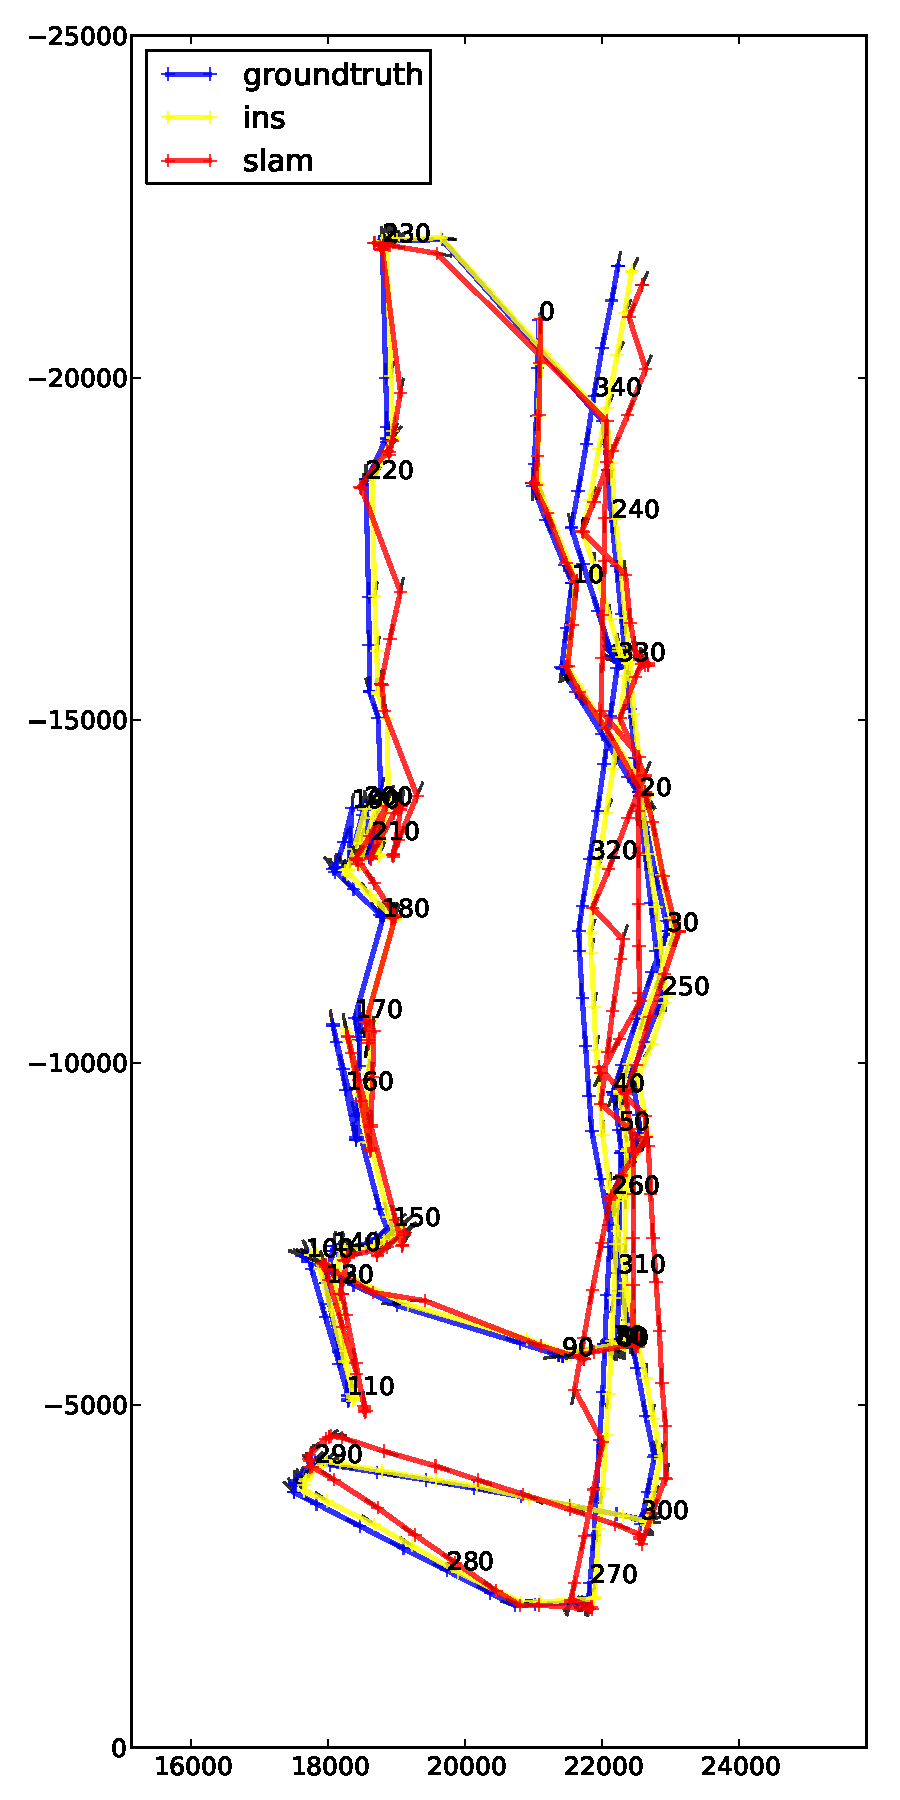
\includegraphics[width=0.3\textwidth]{images/experiment/map1/trace.pdf}
		\label{fig:apx:map1-paths}
	}
	\subfigure[The path of the robot according to SLAM, with associated uncertainty ellipsis. The error is plotted with yellow circles if there was infinite error (no matches at all).]{
		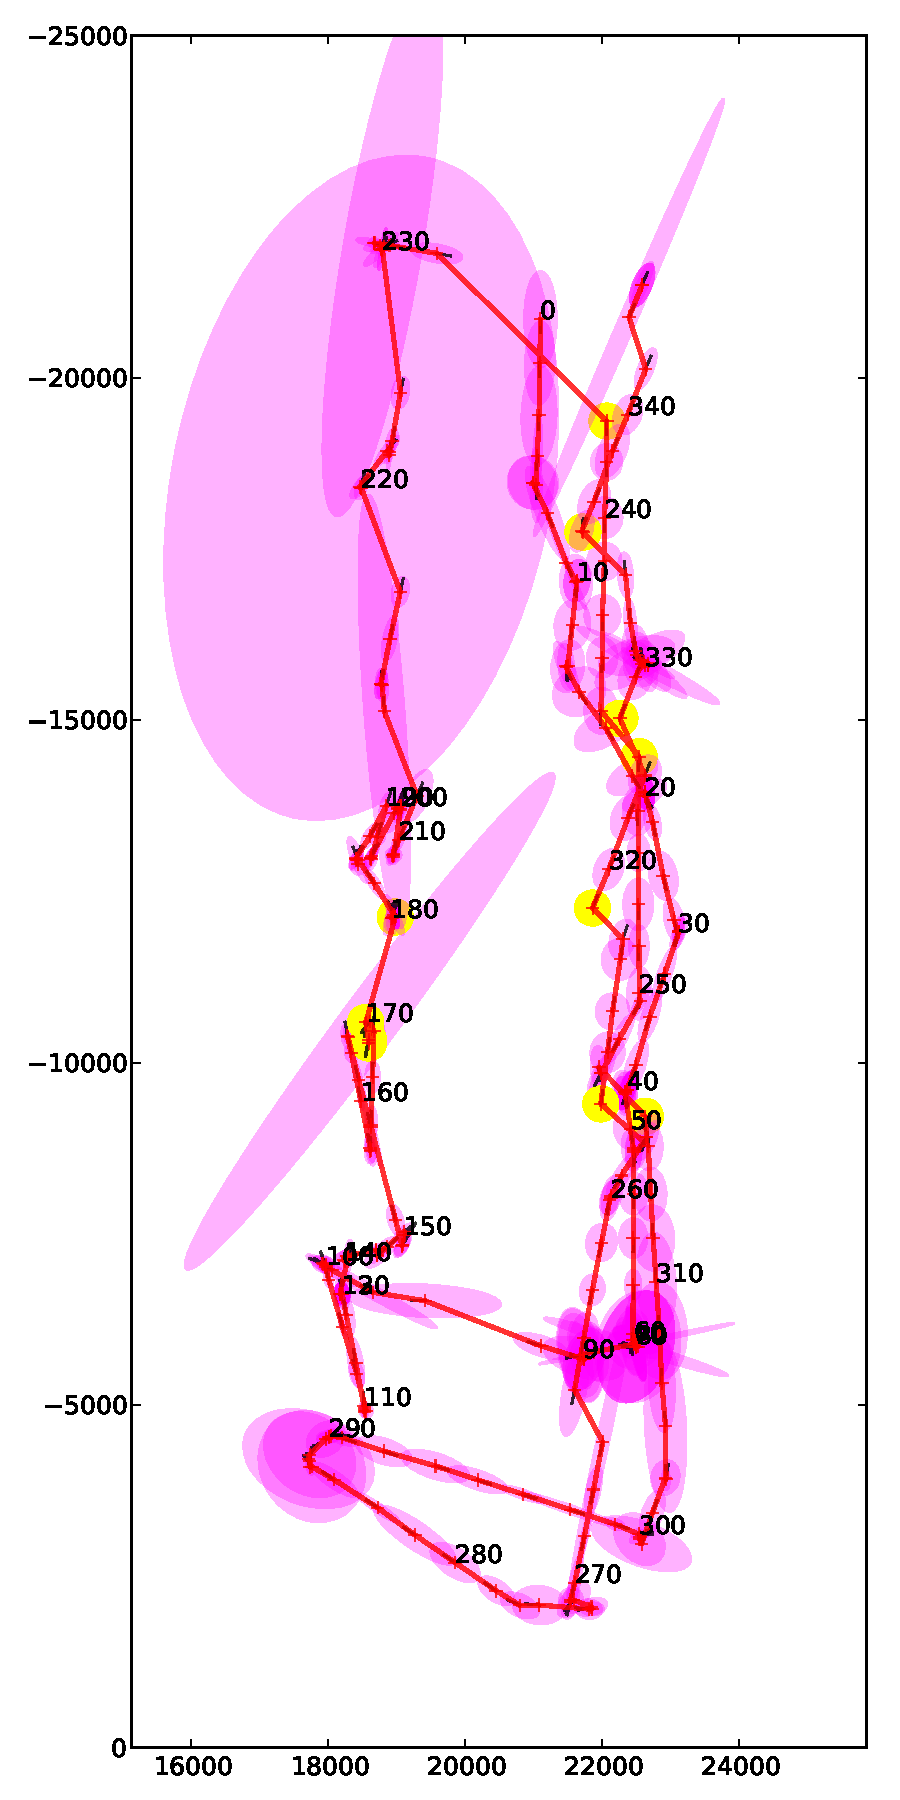
\includegraphics[width=0.3\textwidth]{images/experiment/map1/slam_covariance.pdf}
		\label{fig:apx:map1-trace}
	}
	\caption{Map 1 paths}
	\label{fig:apx:map1}
\end{figure}

\begin{figure}[ht]
	\centering
	\subfigure[Piece 1: $0 \le t \le 65$]{
		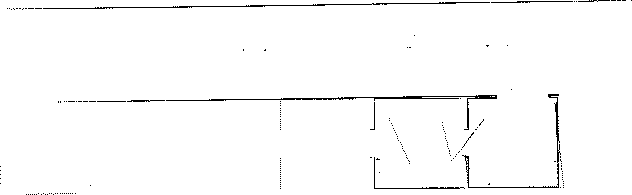
\includegraphics[resolution=180]{images/experiment/map1/maps/part-0-65-1.png}
	}
	\\
	\subfigure[Piece 2: $69 \le t \le 95$]{
		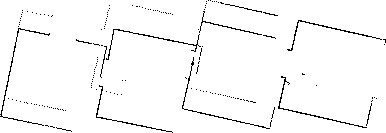
\includegraphics[resolution=180]{images/experiment/map1/maps/part-69-95-1.png}
	}
	\\
	\subfigure[Piece 3: $97 \le t \le 102$]{
		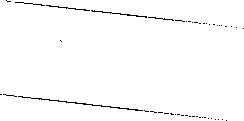
\includegraphics[resolution=180]{images/experiment/map1/maps/part-97-102-1.png}
	}
	\qquad
	\subfigure[Piece 4: $104 \le t \le 112$]{
		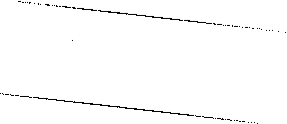
\includegraphics[resolution=180]{images/experiment/map1/maps/part-104-112-1.png}
	}
	\\
	\subfigure[Piece 5: $114 \le t \le 158$]{
		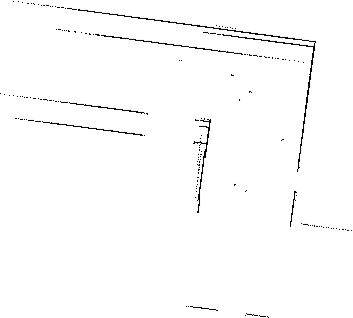
\includegraphics[resolution=180]{images/experiment/map1/maps/part-114-158-1.png}
	}
	\\
	\subfigure[Piece 6: $160 \le t \le 163$]{
		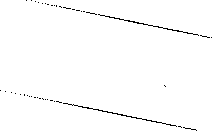
\includegraphics[resolution=180]{images/experiment/map1/maps/part-160-163-1.png}
	}
	\qquad
	\subfigure[Piece 7: $165 \le t \le 167$]{
		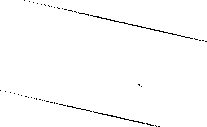
\includegraphics[resolution=180]{images/experiment/map1/maps/part-165-167-1.png}
	}
	\\
	\subfigure[Piece 8: $169 \le t \le 174$]{
		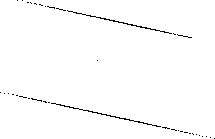
\includegraphics[resolution=180]{images/experiment/map1/maps/part-169-174-1.png}
	}
	\qquad
	\subfigure[Piece 9: $176 \le t \le 182$]{
		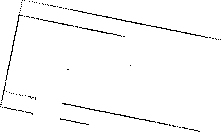
\includegraphics[resolution=180]{images/experiment/map1/maps/part-176-182-1.png}
	}
	\caption{Map 1 parts}
	\label{fig:apx:map1-pieces}
\end{figure}

\begin{figure}[ht]
\vspace*{-2.5cm}
\makebox[\textwidth]{
	\subfigure[step 1]{
		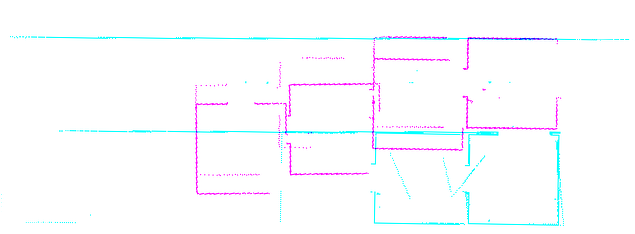
\includegraphics[resolution=180]{images/experiment/map1/result/step1c.png}
	}
	\subfigure[step 2]{
		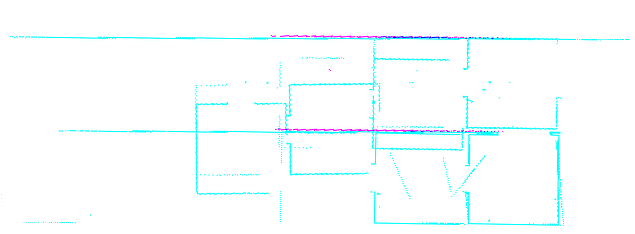
\includegraphics[resolution=180]{images/experiment/map1/result/step2c.png}
	}
} \\
\makebox[\textwidth]{
	\subfigure[step 3]{
		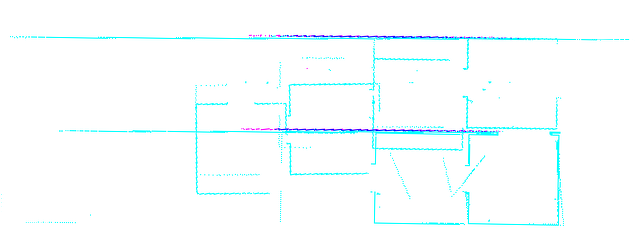
\includegraphics[resolution=180]{images/experiment/map1/result/step3c.png}
	}
	\subfigure[step 4]{
		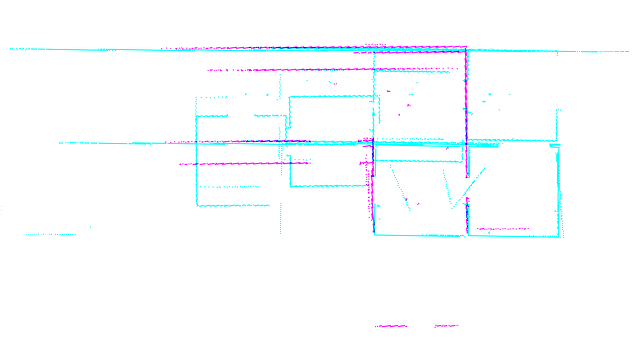
\includegraphics[resolution=180]{images/experiment/map1/result/step4c.png}
	}
} \\
\makebox[\textwidth]{
	\subfigure[step 5]{
		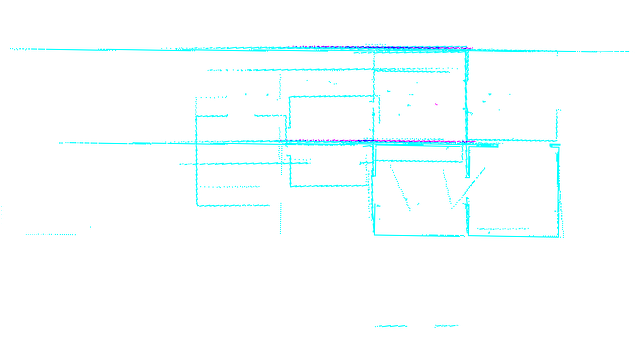
\includegraphics[resolution=180]{images/experiment/map1/result/step5c.png}
	}
	\subfigure[step 6]{
		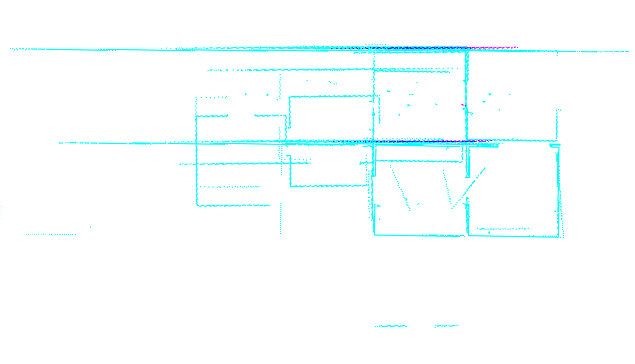
\includegraphics[resolution=180]{images/experiment/map1/result/step6c.png}
	}
} \\
\makebox[\textwidth]{
	\subfigure[step 7]{
		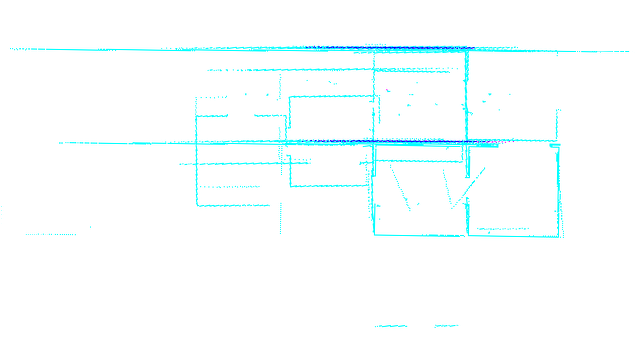
\includegraphics[resolution=180]{images/experiment/map1/result/step7c.png}
	}
	\subfigure[step 8]{
		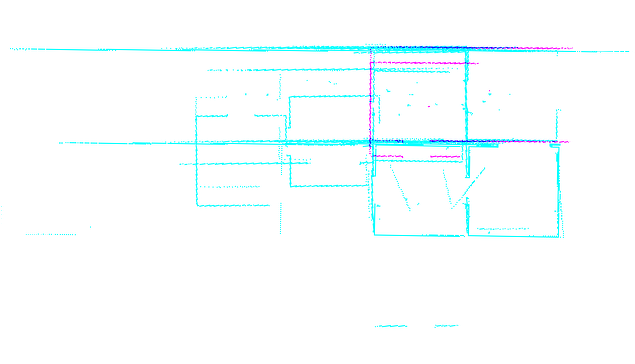
\includegraphics[resolution=180]{images/experiment/map1/result/step8c.png}
	}
} \\
\caption{Map 1 stitching steps}
\label{fig:apx:map1-steps}
\end{figure}


\section{Experiment 2}

\begin{figure}[ht]
	\vspace*{-2.5cm}
	\centering
	\subfigure[Piece 1: $0 \le t \le 291$]{
		\makebox[\textwidth]{
			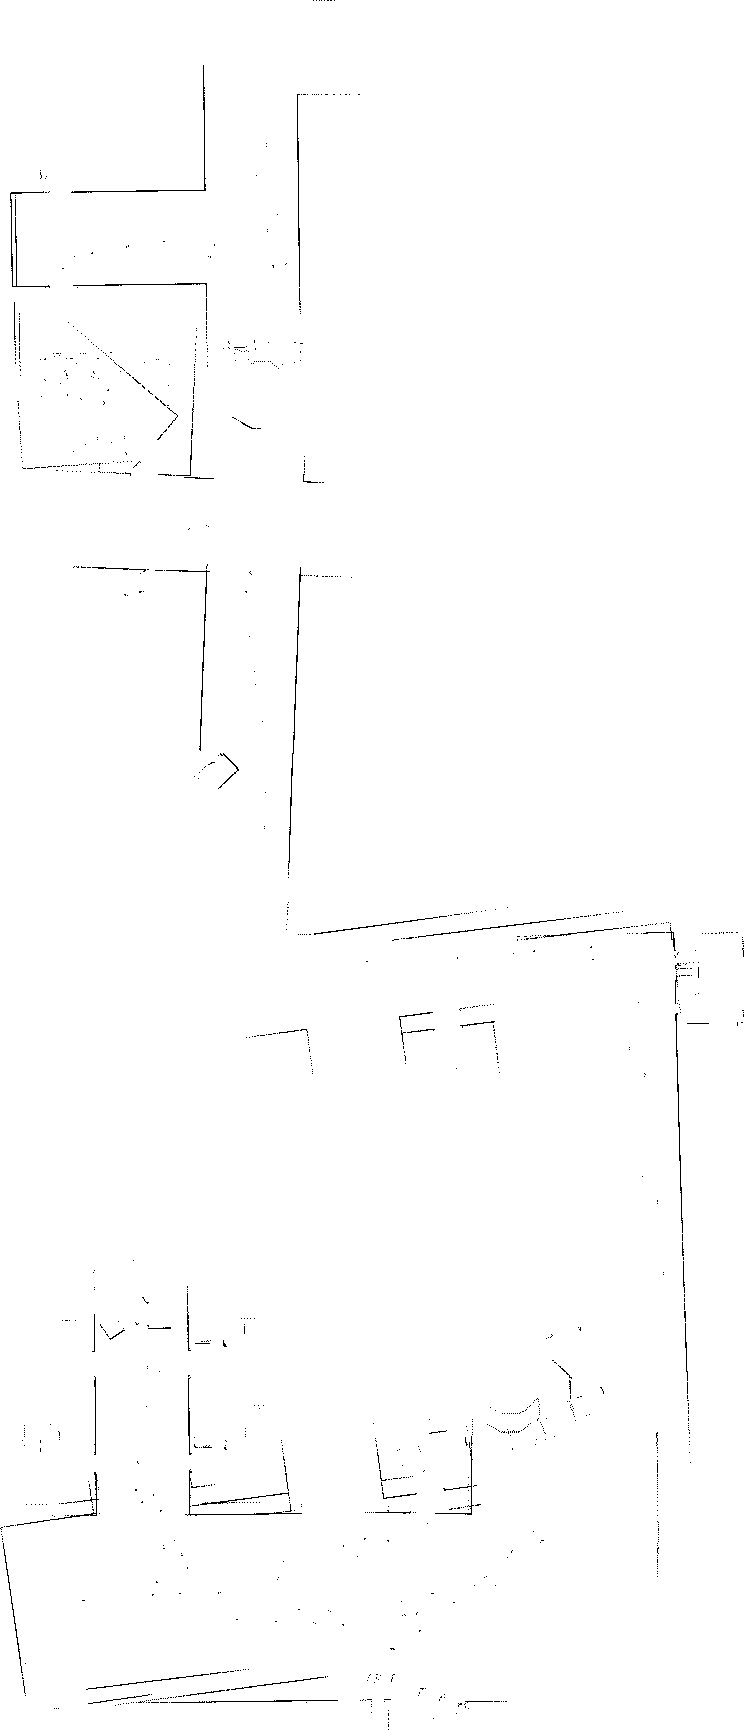
\includegraphics[resolution=340, angle=-90]{images/experiment/map3/maps/map3-part1.png}
		}
	}\\
	\subfigure[Piece 2: $297 \le t \le 747$]{
		\makebox[\textwidth]{
			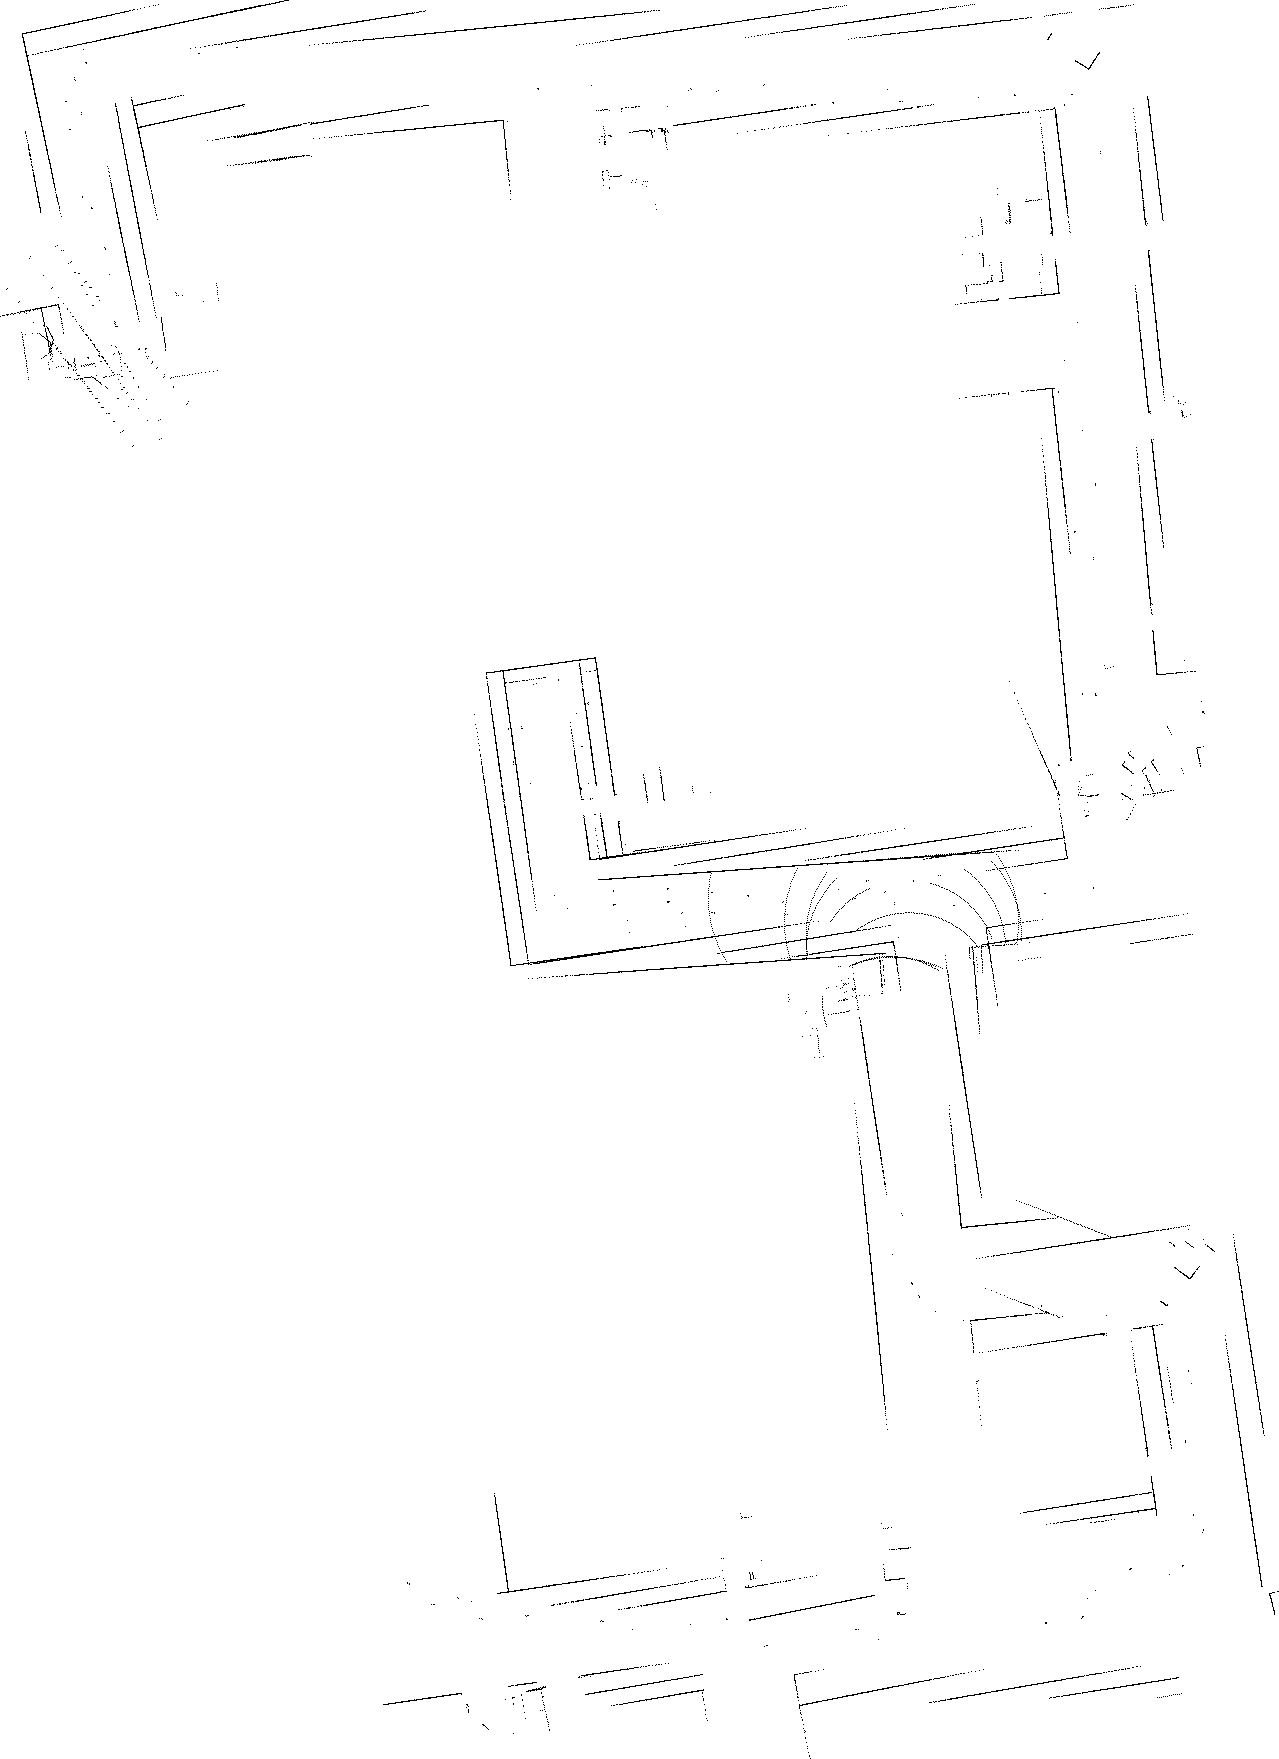
\includegraphics[resolution=340, angle=-90]{images/experiment/map3/maps/map3-part2.png}
		}
	}\\
	\subfigure[Piece 3: $750 \le t \le 1002$]{
		\makebox[\textwidth]{
			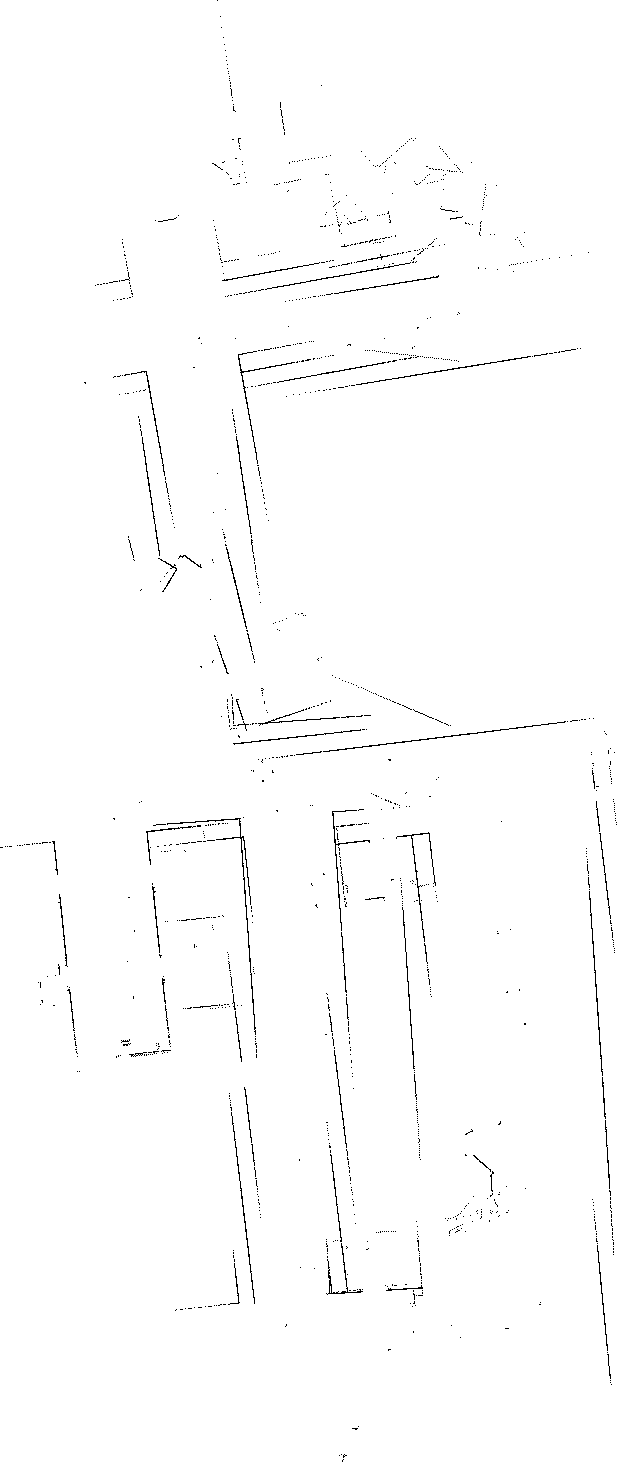
\includegraphics[resolution=340, angle=-90]{images/experiment/map3/maps/map3-part3.png}
		}
	}
	\caption{Map 2 parts}
	\label{fig:apx:map3-pieces}
\end{figure}


\begin{figure}[ht]
	\vspace*{-2.5cm}
	\centering
	\subfigure[After merging piece 1 and 2]{
		\makebox[\textwidth]{
			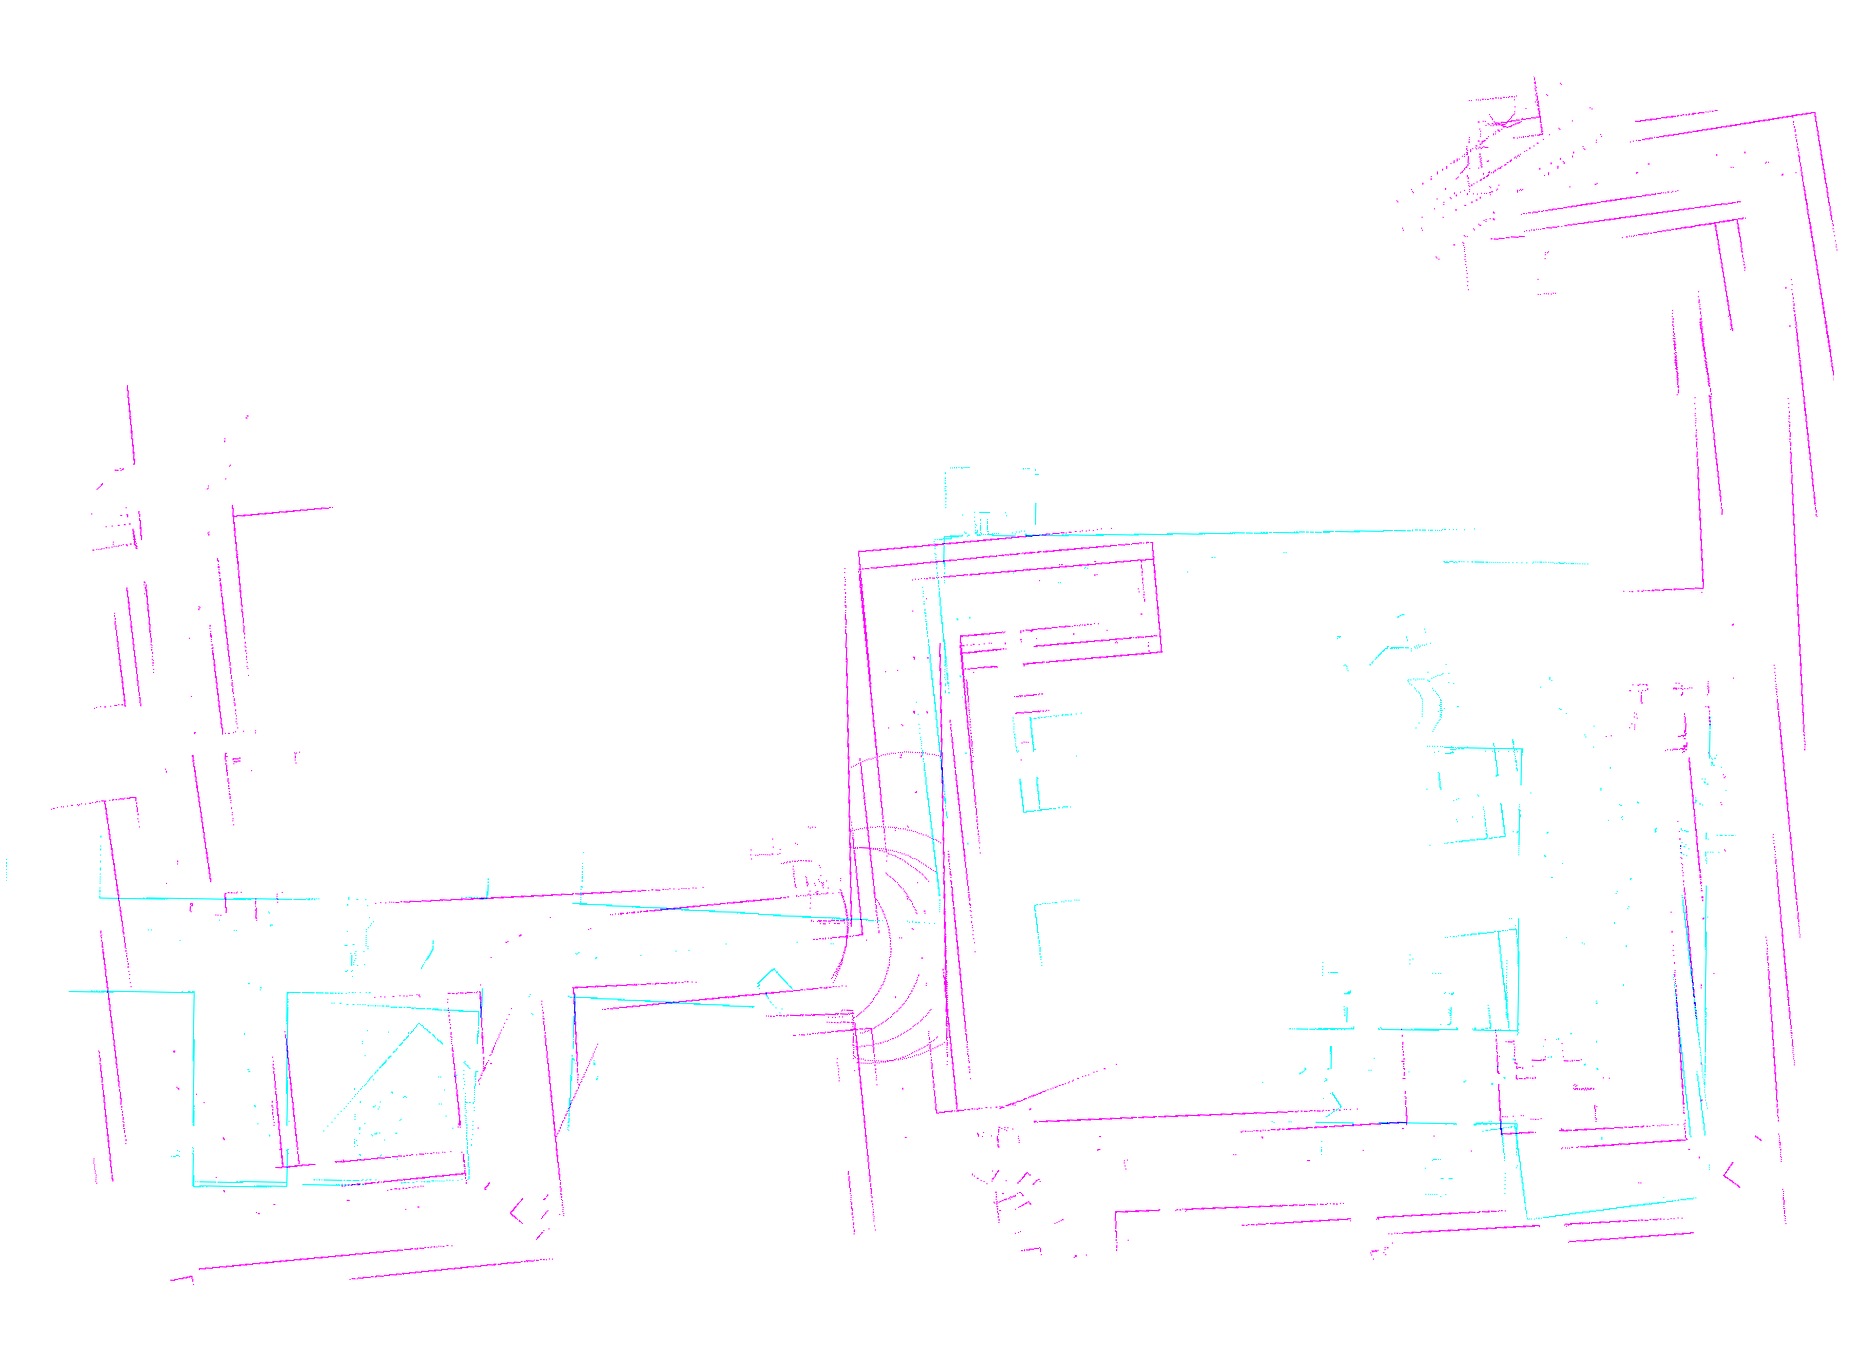
\includegraphics[resolution=380]{images/experiment/map3/result/step1c.png}
		}
	}\\
	\subfigure[Adding piece 3]{
		\makebox[\textwidth]{
			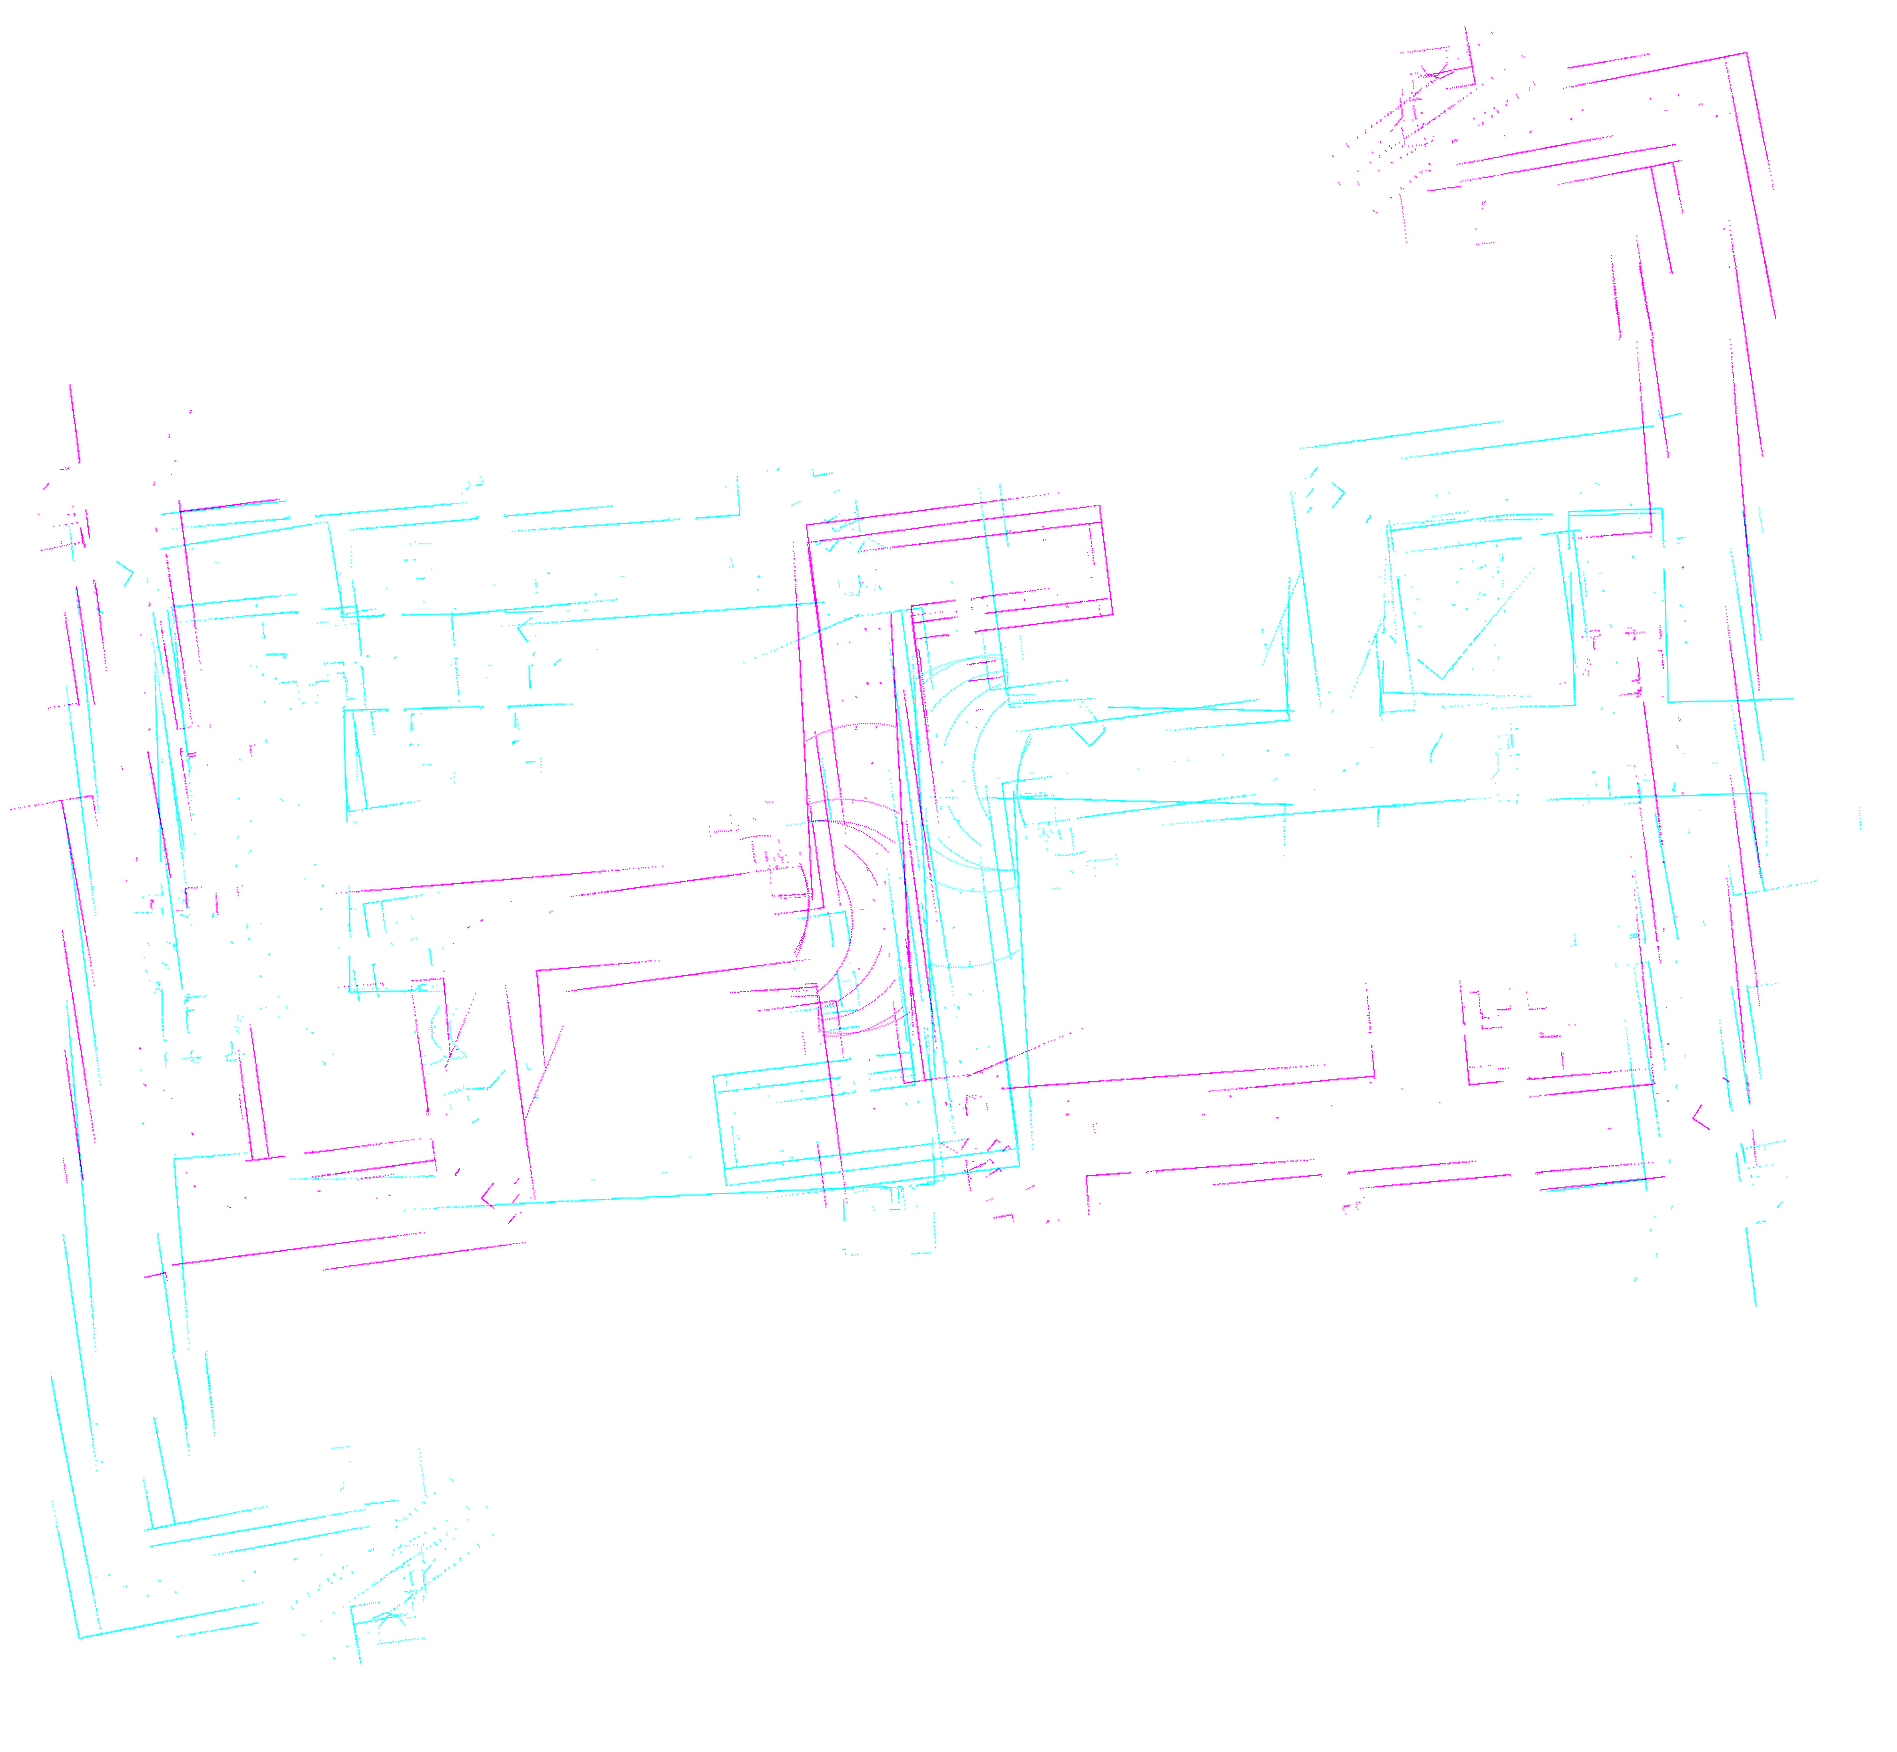
\includegraphics[resolution=380]{images/experiment/map3/result/step2c.png}
		}
	}
	\caption{Map 2 results}
	\label{fig:apx:map3-results}
\end{figure}


%TODO: Show map pieces and stitching results

\section{Experiment 3}
\begin{figure}[ht]
	\vspace*{-2.5cm}
	\centering
	\subfigure[Piece 1]{
		\makebox[\textwidth]{
			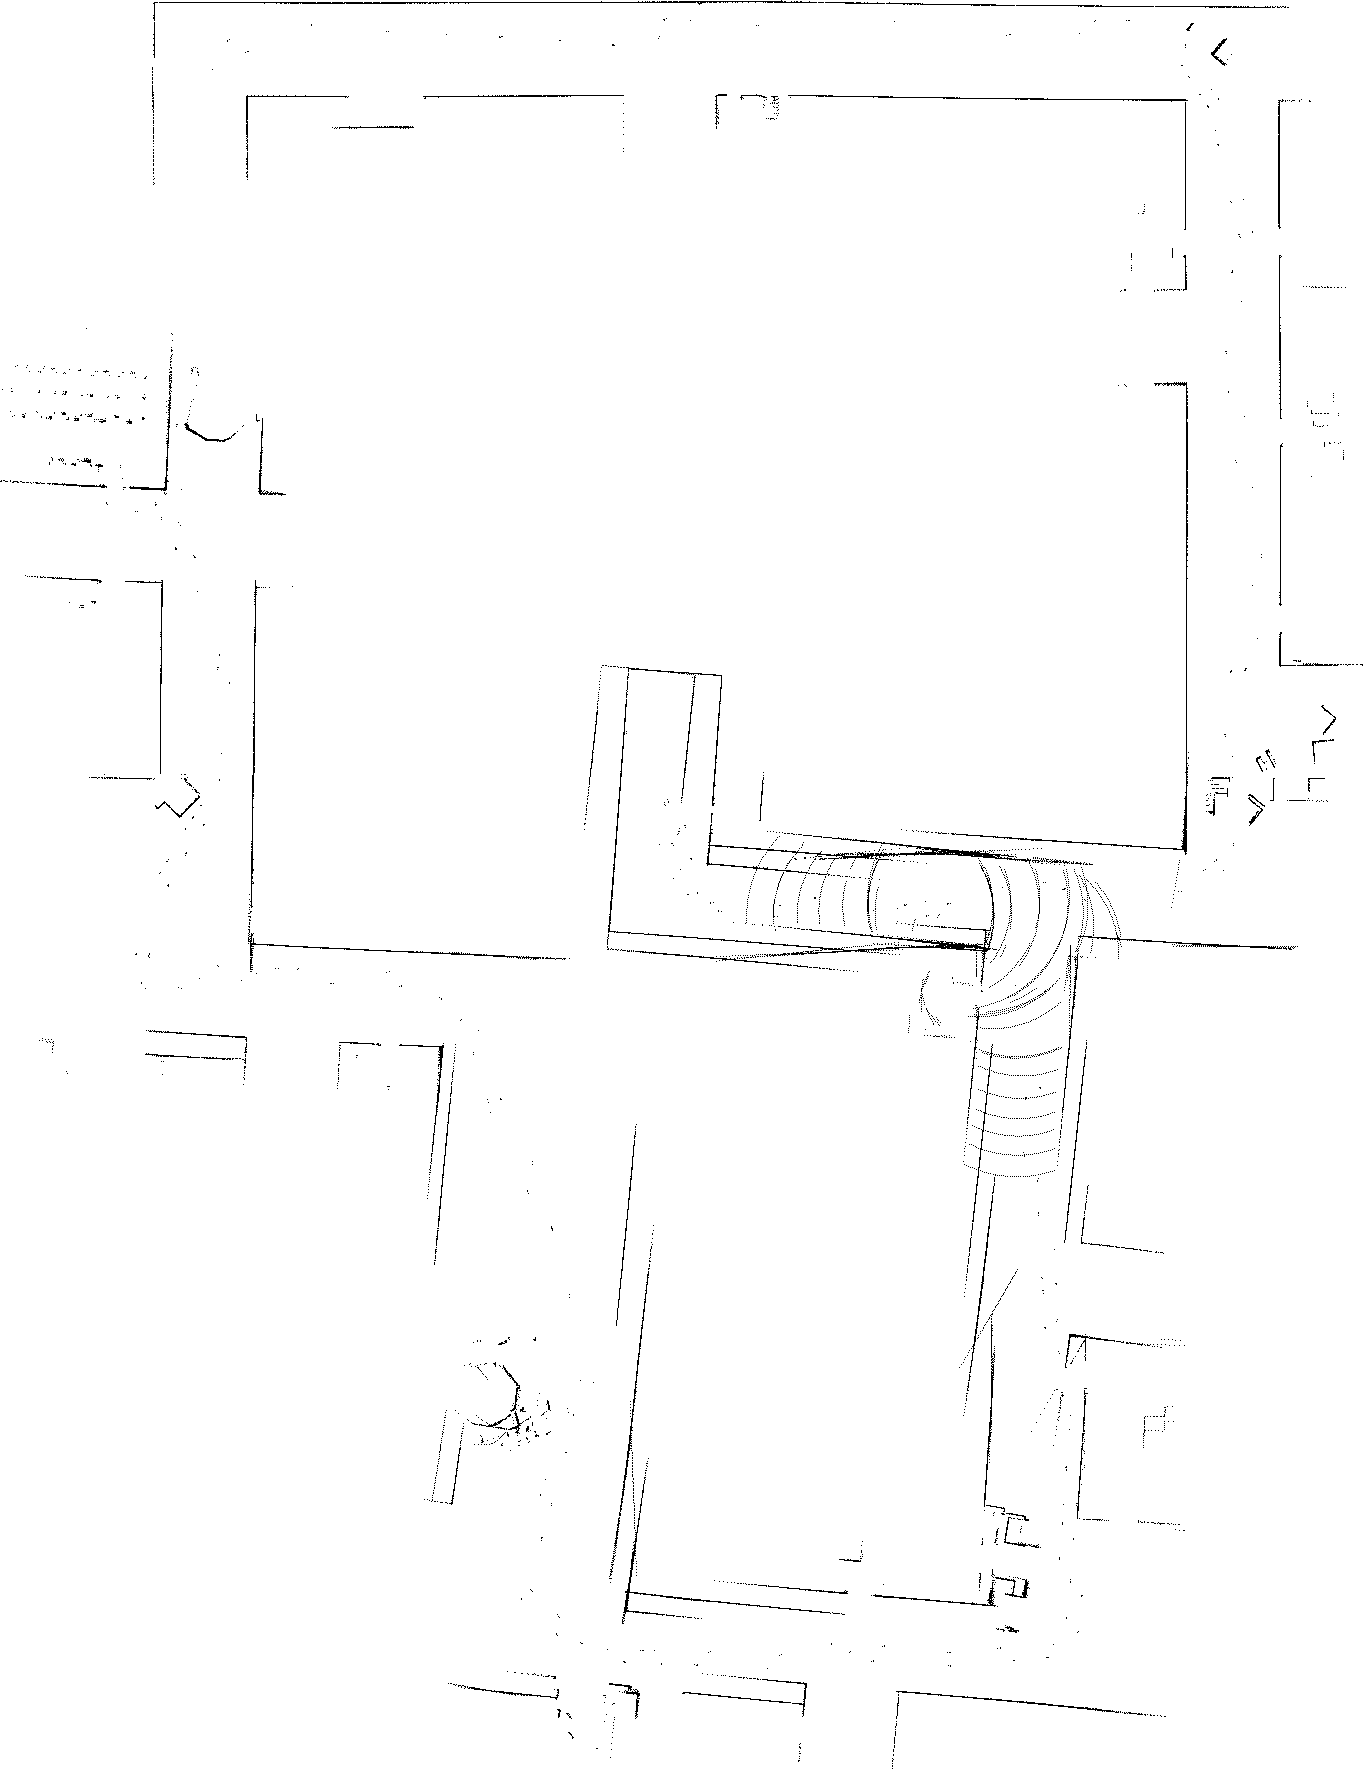
\includegraphics[width=0.8\textwidth, angle=-90]{images/experiment/map4/part1-1.png}
		}
	}\\
	\subfigure[Piece 2]{
		\makebox[\textwidth]{
			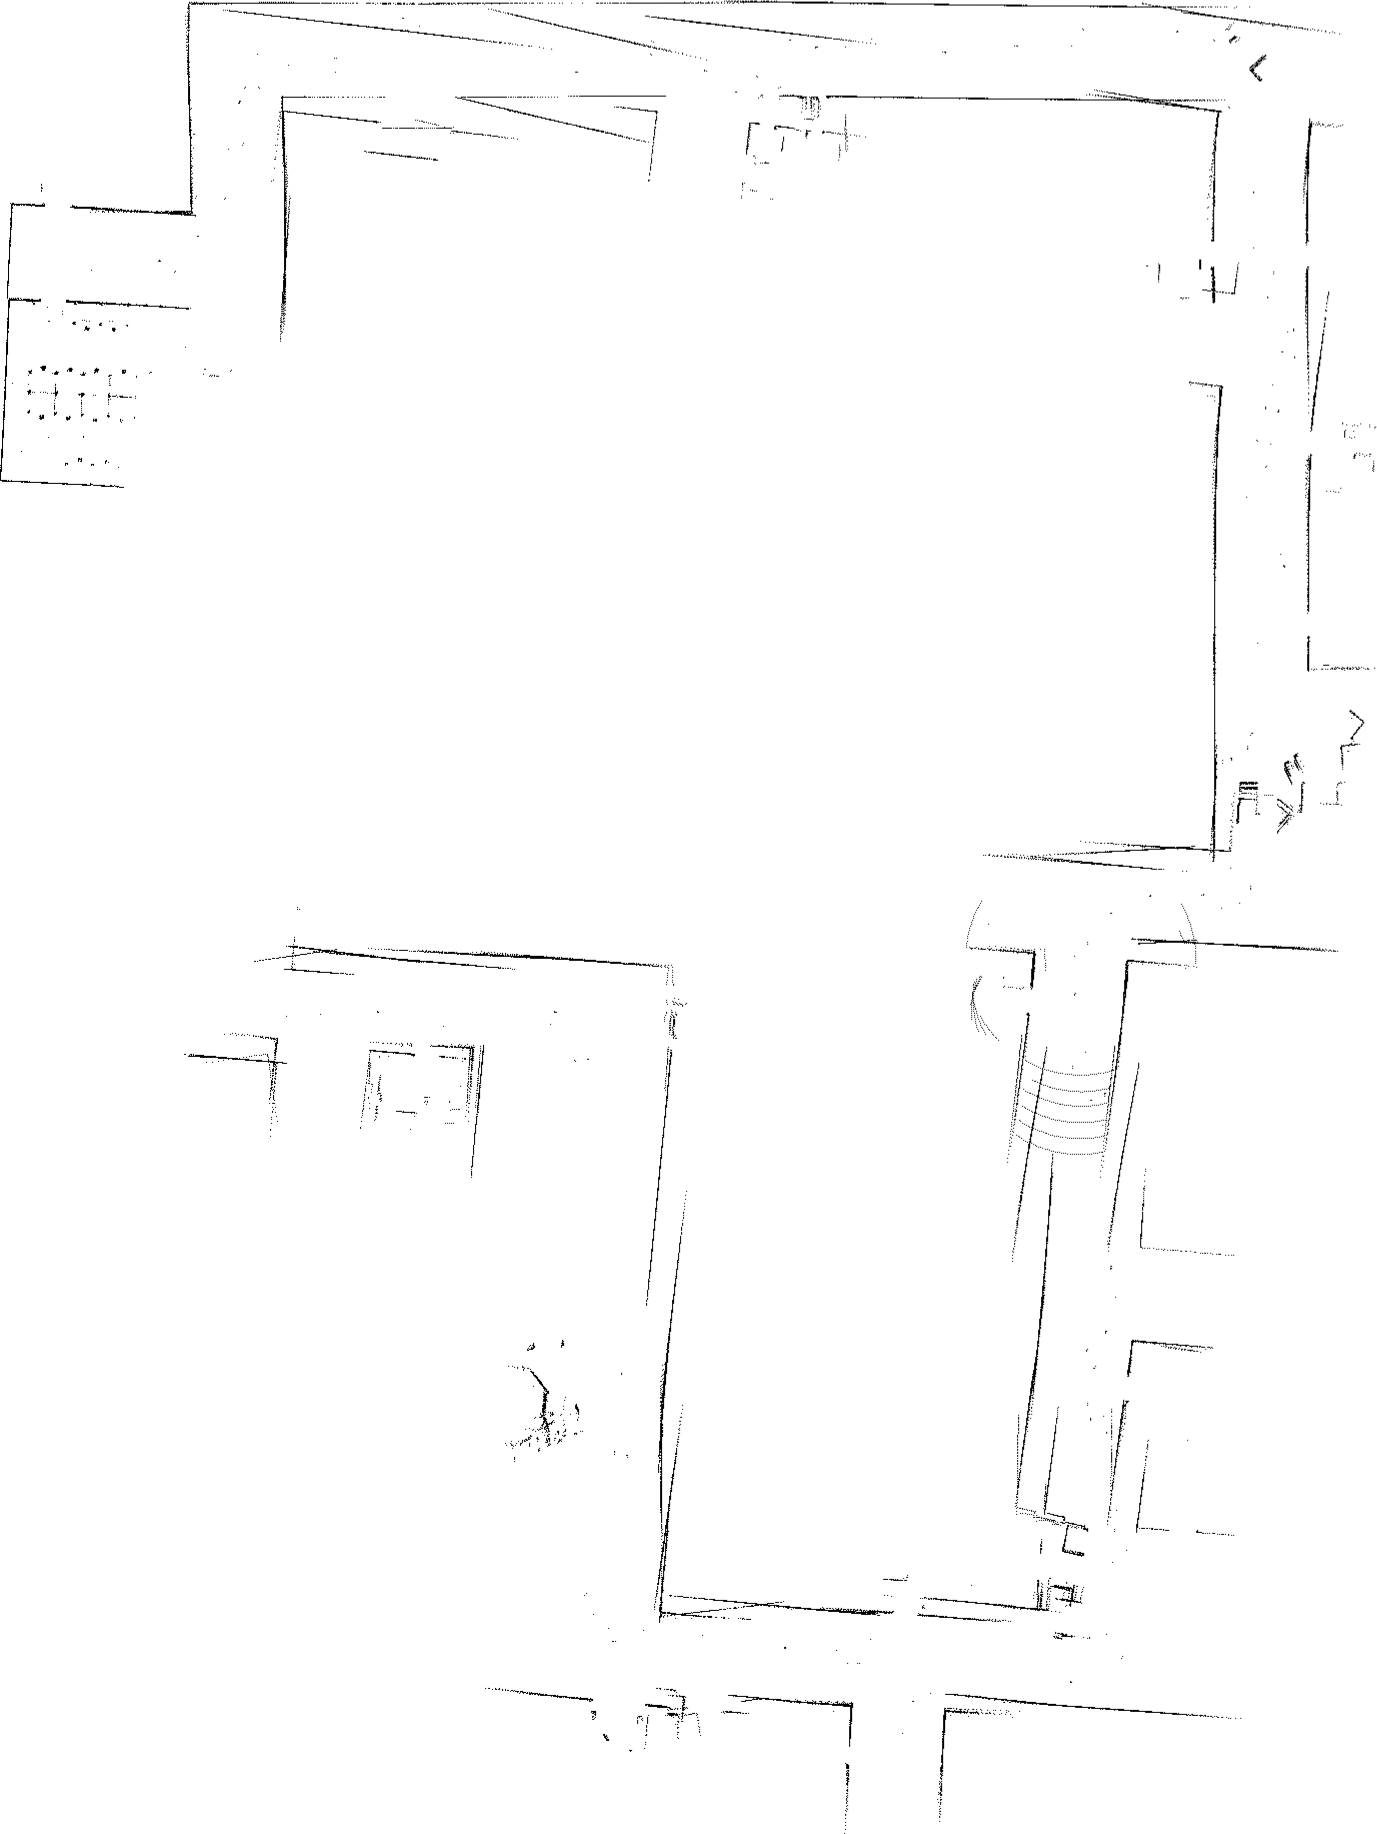
\includegraphics[width=0.8\textwidth, angle=-90]{images/experiment/map4/part2-1.png}
		}
	}
	\caption{Map 3 parts}
	\label{fig:apx:map4-pieces}
\end{figure}


\begin{figure}[ht]
	\centering
	\makebox[\textwidth]{
		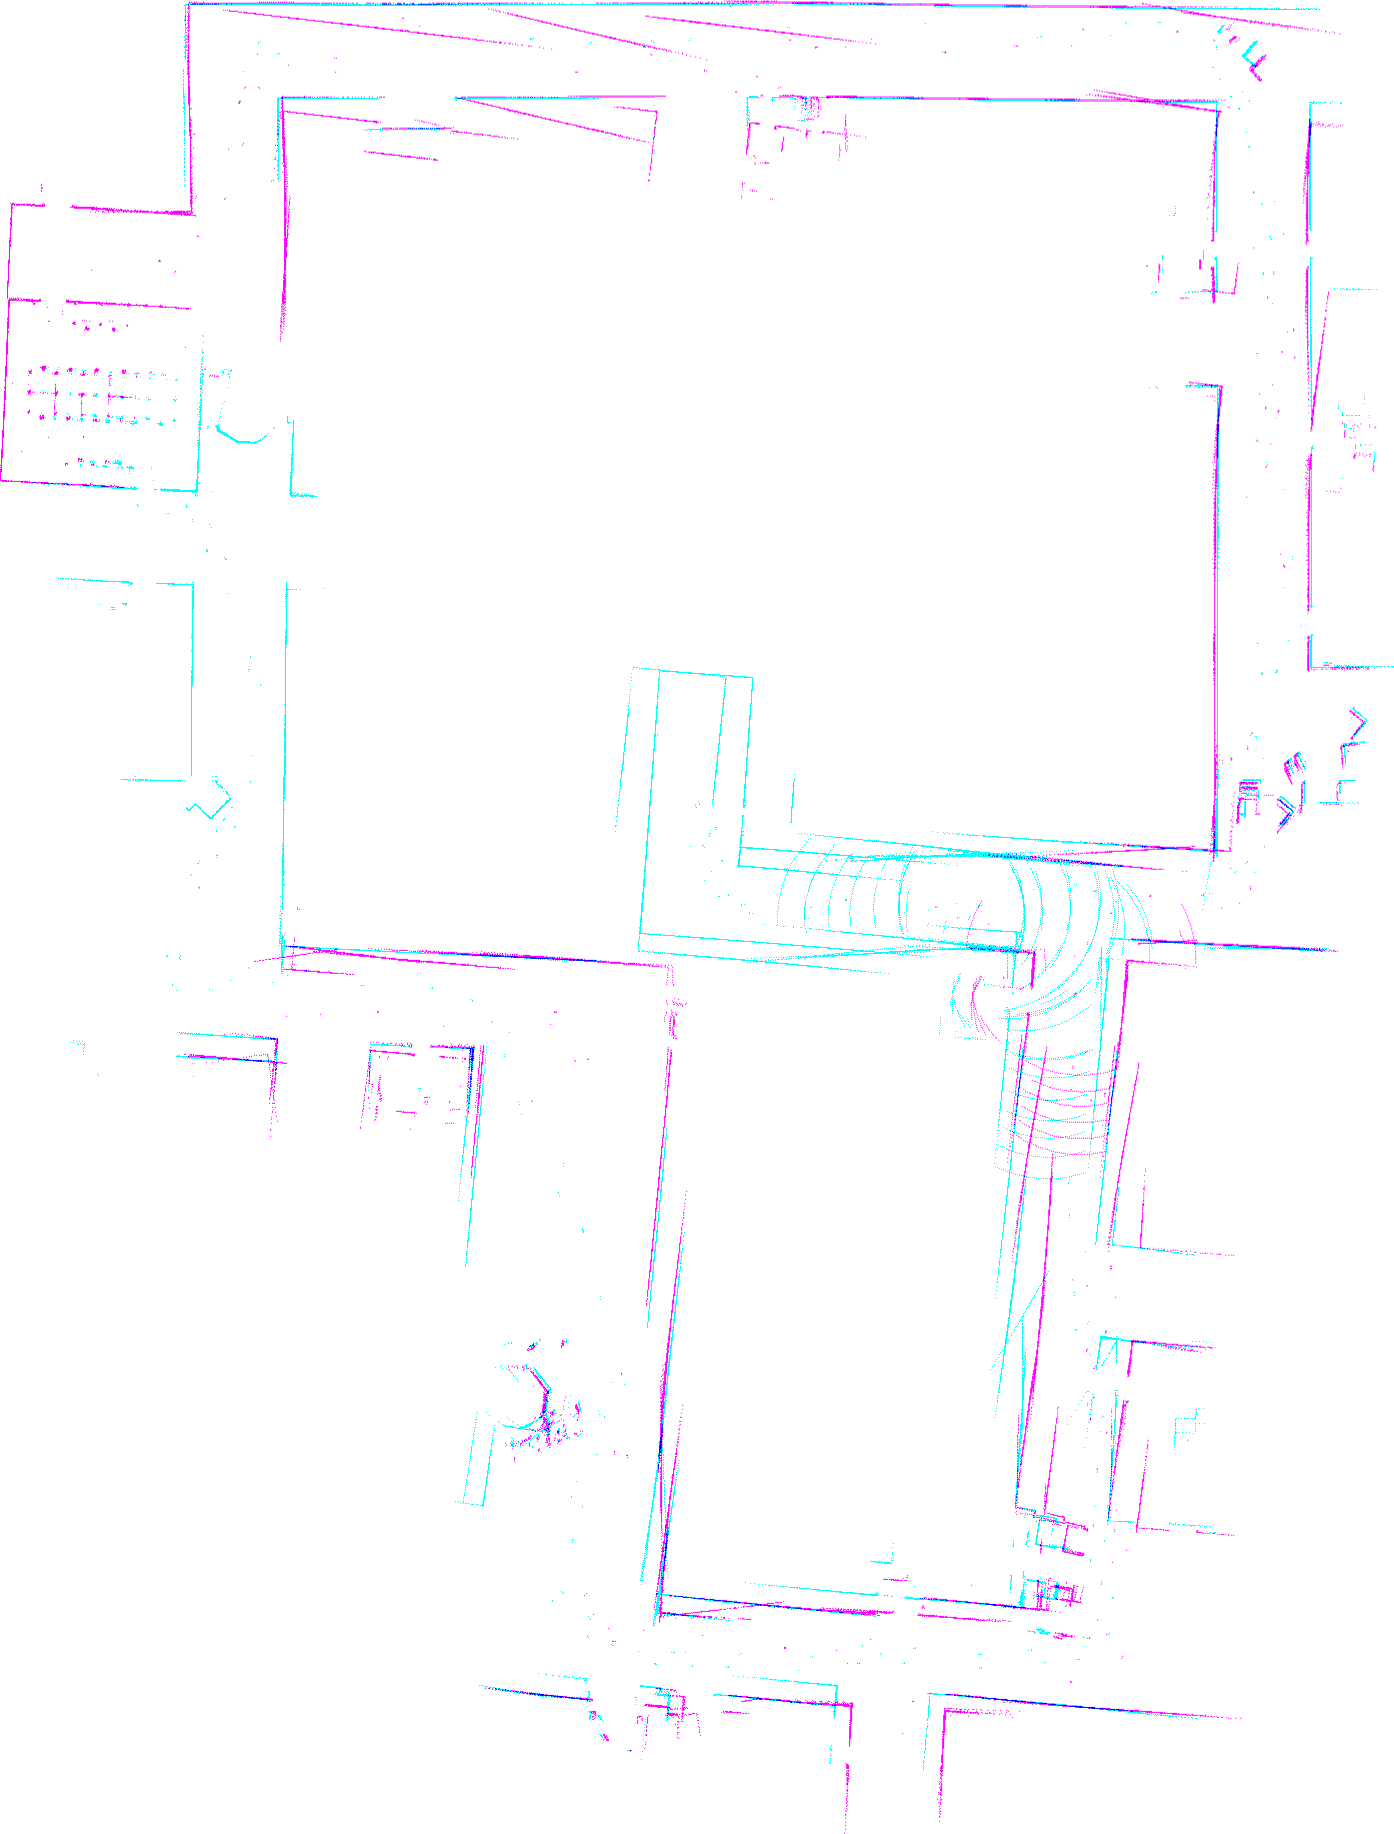
\includegraphics[width=\textwidth, angle=-90]{images/experiment/map4/results/result_color_0.png}
	}
  \caption{Map 3 results}
  \label{fig:map4-results}
\end{figure}



% TODO: Show map pieces, and stitching results
